\documentclass{article}
\usepackage{comment}
%\usepackage{natbib}
\usepackage{graphicx}
\usepackage[natbibapa]{apacite}
\begin{document}

\title{Choosing the Choice: Reflections on Modelling Decisions and Behaviour in Demographic Agent-Based Models}
\author{Jonathan Gray \and Jason Hilton \and Jakub Bijak}

\maketitle

\section{Introduction}
\label{sec:intro}

As demonstrated throughout this Special Issue, agent-based models have become important tools with which demographers can study mechanisms of social reality, enhancing the analysis of population processes with multi-level influences, feedback effects, the presence of networks and interactions. Still, the related methodology remains under development: in particular, as evident in the nascent demographic agent-based literature, there is hardly any discussion on operationalising the actual decision making processes, through which the agents could acquire some more agency beyond reflexive reactions to simulated stimuli. 

In this research note, we discuss the challenges of choosing an appropriate model of choice in the context of decision making in agent-based demography. The argument is illustrated by examples related to demographic agent-based models, with focus on migration. In particular, in Section \ref{sec:context_matters} we elaborate on the role of the context of the decision processes. In Section \ref{auxiliary-factors-in-modelling-decisions}, we discuss some specific aspects of the mechanics of choice: time, heterogeneity of agents, as well as the choice between the choice models as such. Finally, in Section \ref{multi-model-approaches-and-modularity}, we conclude with a list of tentative recommendations for further work in the area, focusing on the mechanisms of decision making, multi-disciplinary approaches, a multi-model framework, and modularity of agent-based modelling.


\section{Context Matters}
\label{sec:context_matters}

This section stresses the axiomatic status of the current models of choice in agent-based simulation, and discusses the numerous interfaces between choice and context at which modelling decisions must be made.

That the context in which a decision is made plays a role in the choice is inarguable: context can strongly influence the decision process itself \citep{Ben-Akiva2012}. The challenge arises in determining what the context is, and having done so, deciding what of it to consider, and how to operationalise it. The former is the easier task, since the context is the universe up to the moment of decision. The latter are more problematic, and the `state of the art' is for now, just that - an art. 


We suggest that inclusion and operationalisation of context are best tackled through an iterative process of development, and evaluation against empirical data. This approach places considerable demands on the modeller in terms of developing the model, but also in exercising their judgement as to what should be included, and identifying where a component should be iterated out. In a sense, this is a similar process to the stepwise approaches commonly used in constructing regression models. Here, however, it is considerably less amenable to automation, both because augmenting a model is time consuming, and because evaluating complex models poses considerable challenges. The challenge of evaluation can be somewhat ameliorated by the use of techniques like sensitivity analysis (see \citet{Thiele2014} for a review of several techniques, and \citet{Oakley2004} for an alternative approach), which can support the modeller in identifying how the individual parameters of a model contribute to overall outputs. This too has limitations, because as we discuss later in relation to heterogeneity in agents (section \ref{heterogeneity-in-decision-strategies}), context can take the form of both process, and parameter.
As a result, the onus remains on the modeller to use their best judgement.

As an example, we might consider social context, and how it is treated in modelling one demographic process. The social context of a decision is a broad sphere touching as it does on social norms, the role of the decision maker's social network, and so forth. Social context, and indeed any context, may interact with decision making by being represented as a parameter to the decision model, or through impacting on the outcome of enacting a decision. Naturally, where the context is an input to the decision model, the modeller must consider whether process it arises from is within the scope of the model, or should be externalised.
Here, we will follow the lead of \citet{Klabunde}, and examine how social context is operationalised when modelling migration. 

The prototypical approach to modelling choice is to employ some form of random utility model (\citet{Baltas2001} have reviewed the key types, in the context of marketing research), where all decision makers consider the same factors in their decision making, and choose between the same options. Considering migration, social networks have a clear role \citep{Epstein2006}, both through social influence on decision making, and in the process by impacting how far a migration decision succeeds. Naturally, the two are not indivisible, since success or failure carries implications for how that actor influences others.

If we limit ourselves further, and consider only how social influence might be modelled, then there are two key questions: what is the unit of influence; and how does influence interact with decision making. It will be useful to address these one at a time, although the two are of course intertwined, since influence is information that affects behaviour. This is also demonstrated by \citet{Mason2007} in their review of models of social influence, where many models treat these aspects in combination.

The flow of influence is synonymous with the flow of information, which has attracted considerable attention in the last few years, with an increasing appreciation of the role of social networks in social influence. Here, rather than the structure over which influence flows, we will focus on what flows over it. 
Where information is transacted, it may be about attitudes, or actions, or outcomes, and can correspond strongly or weakly to the truth. The mechanics of flow can also vary considerably, for example transmission might occur only between direct links, or be passed along many, and may pass in only a single direction.

The distinction between acts, and attitudes is an interesting one largely unexplored in this arena. Typically, we observe the actions of others, rather than getting accurate insight into their reasoning. Where actions are what agents observe, their function is usually socially normative, for example in \citeauthor{Silveira2005}'s (\citeyear{Silveira2005}) model of rural-urban migration, an agent's utility is partially a function of how similar their behaviour is to that of their neighbours. The contrasting approach is to communicate a representation of the attitudes of the agent, used by \citet{Espindola2006} in an earlier simulation of rural-urban migration, where agents compare `satisfaction'.

Neither approach is a complete account. While mimicry seems to be fundamental to many aspects of human behaviour \citep{Chartrand1999}, we are not simply impersonators and instead interpret the actions of others. Absent telepathy however, we can only draw inferences based on observation of their actions\footnote{Which may well include communicating about their internal state.}. A potential approach to this might be one similar to that of \citet{Jern2011a} who propose an inverted generative model\footnote{A generative model produces decisions, given preferences over outcomes. The inversion provides estimates of preferences, given observed decisions.} to explain how people might translate observed behaviour into preferences, although this presages a utility type mechanism for decision making. This also has implications for more high level models of the interaction between context and decision making process, for example that of \citet{Ben-Akiva2012}, where there are explicit models of the interaction between context and choice. An inverted model which does not sufficiently capture the context in which an agent's decision making took place, i.e. the observing agent is underinformed about inputs to the other's decision process, or constraints on their actions, may well lead to faulty inferences about what drove their behaviour. Although this is realistic, in that our own inferences about the motivations of others are not always accurate, it may not be desirable in all models.

The other usual interpretation of social information flow is as transmission of information about the state of the world, for example information about expected income, as in models by \citet{Filho2011}, and \citet{Klabunde2014}.  Relating this back to our previous mention of faulty inference, this raises the issue of decision making in an uncertain world, since there is no guarantee that information is accurate. In both models, agents take the average incomes of others in their social network as their expected income were they to relocate. Although some distortion may be introduced by the limited sample, the reported income of other agents is perfectly accurate. 
A potential extension might be to consider inaccuracy arising from cognitive bias; for example, \citet{Mather2000} found that people distorted their recollections in favour of the choices they had made, suggesting that agents might exaggerate their success. Alternatively, \citet{McKenzie2013} found that potential migrants had unrealistically negative expectations about earnings and employment. They suggest this may partly arise from attempting to reduce demands for remittances, i.e. agents underreport their incomes. In either case, this suggests that information transmission is not always simply a passive process.

\citeauthor{McKenzie2013} also suggest that overweighting of negative experiences plays a role, which demonstrates the importance of considering how information is incorporated into the decision process. In this case the suggestion is that another cognitive bias, loss aversion, is a salient feature. This could be reflected by using a decision model explicitly incorporates loss aversion, for example Prospect Theory \citep{Kahneman1979}, or Cumulative Prospect Theory \citep{Tversky1992}. Both variants of Prospect Theory are intended to mimic human decision making, by distorting the perception of high and low probabilities towards certainty, and shifting the value of gains and losses such that large gains are progressively less significant, and losses more so. 
The wider implication is that social information flow may be distorted at the source, or through interpretation, and that agent-based models are uniquely suited to capture this.  Other approaches to decision models are available, for example heuristic methods \citep{Gigerenzer1996}, which emphasise the bounded rationality of human decision making, and Bayesian approaches, which address learning as a component of the decision process \citep{Robbins1964}. In an agent-based modelling context, \citet{Gray2016} have contrasted Bayesian, heuristic, and Cumulative Prospect Theory approaches in a simulation of alcohol misuse disclosure among pregnant women.

As we have intimated, we believe that introducing such additional complications to a model necessitates an iterative approach. We also believe that the implementation model of decision making should be treated as a feature to iterate on, and that different models should be contrasted against one another. This suggests that modularity should be a key consideration in model design, to support the modeller in evaluating the relative merits of different decision models, given the purpose of the overall model.

The diversity of approaches to this single issue is reflective of the open ended nature of agent-based modelling. A recurring feature however, is that an appreciation is needed of the multiple roles of contexts in decision making. Interpersonal context, for example, is a critical feature of information transmission, but also plays a role in the subjective value of outcomes. This is a challenge, since it is not clear that the two are readily separable, and our understanding of interpersonal context is incomplete.
However this presents us with great opportunity, in using simulation to expand our understanding both of the role of social processes, and their mechanics; and in following the example of \citeauthor{Tversky1992} by forging inter-disciplinary collaborations with experts in the micro-domain of behaviour.




\section{Auxiliary factors in modelling
decisions.}\label{auxiliary-factors-in-modelling-decisions}

This section focuses on two auxiliary model elements that are often understandably overlooked in implementations of agent decision models, but are also key assumptions. The first is the treatment of time in models of decision making, while the second is the extent to which individual agents differ in their approaches to making decisions in the same context.

\subsection{Time}\label{time}

Time is explicitly represented in almost all agent-based models, either in discrete or (pseudo) continuous form, in order to allow the dynamic unfolding of the modelled processes by `stepping' from one time-step to the next (or between time-ordered events in continuous-time discrete-event simulation). However, time often  does not enter into the decision making process of the simulated individuals, in that agents do not differ in their preferences between rewards realised immediately and equivalent rewards realised at some point in the future. 

There are many good reasons why ignoring time in models of decision making might be valid or even desirable (and, as modellers, we have often done so). As was noted above, the context and research question must of course inform modelling decisions. It may be that the decisions in question have only short-term consequences, and so a detailed consideration of how agents treat time in their decision making be completely superfluous.

That said, as demographers, we are generally concerned with decisions which affect the life-course. These necessarily have consequences which extend far beyond the present. For example, the decision to have a child may affect not only a parent's immediate satisfaction with life, labour market participation, income streams, consumption and so forth, but will continue to do so for the rest of their life. Future `opportunity costs' must also be borne in mind: taking such a decision now may widen or narrow future options in various other areas of life. Similar considerations are salient for migration and partnership decisions, and indeed for many other demographic and social phenomena, for which the questions of time and sequencing of events tend to be too often ignored (see \citet{Abbott2001} for an excellent overview).

This assumed sensitivity of demographic decision-making to the horizons over which the resultant costs and benefits are realised suggests that we should at least acknowledge what assumptions we make about how people value present and future rewards. The flexibility of agent-based models suggests that are is also scope to examine the effect of decision models including time preference. A brief summary of some current thinking on time-dependence in decision making follows; including such models in demographic models will certainly be challenging, and in many cases impossible, but being aware of the potential problems with making simplifying assumptions about treatment of time in decision models is valuable, and at least helps a modeller anticipate when such assumptions may fall down and why.

Many economic models do of course include time preference in decision making through the use of discounting; in migration modelling, this element is already present in the neoclassical framework, whereby the potential future gains from migration are discounted (see \citet{Massey1993} for an overview). This approach assumes that rewards received in the present are valued more highly by decision makers than those that will only be realised later. The most common functional form for such discounting is the exponential \citep{ODonoghue2000}:

\[
U^{t}(u_t, u_{t+1},\dots,u_T ) = \sum_{\tau=t}^{T} u_{t+\tau}\delta^{\tau}
\]

Here, \(U^t\), denoting present utility at time \(t\), is a function of the stream of individual rewards \(u_t\) at each time point, weighted  according to \(\delta^{\tau}\), with \(\delta\) being the discounting factor. This form has nice properties in that it is time-consistent; agents who prefer one option over another today will do so until the reward has been realised. As an example, consider a utility maximising migrant who optimises their lifetime utility by either settling in the country to which they have migrated, or saving for a time and then returning home in order to spend such savings. If such a migrant discounts future rewards exponentially, then they will make a choice between these alternatives based on the rate of discount and the value of their savings at home relative to consumption in the host country. Crucially, if the situation does not change, such a decision will remain optimal throughout the agents lifespan.

However, experimental evidence for both humans and animals suggests that this is not how time discounting is actually practised \citep{Boyer2008}. While we do prefer rewards now to those later, we do not do so in a consistent manner; preference orderings may change as we move forward in time. The functional form suggested by this sort of behaviour is hyperbolic \citep{Benhabib2010}:

\[
U^{t}(u_t, u_{t+1},\dots,u_T ) = \sum_{\tau=t}^{T} \frac{ u_{t+\tau}}{1+\delta\tau}
\]


%\citet{Sozou1998} provides an interesting interpretation of this behaviour which allows it to be recast as rational. If a reward can be considered as uncertain and subject to constant hazard of being `lost', then we obtain an exponential function, as is well known. If the underlying hazard is also unknown, and an agent continuously updates an estimate of it according to Bayes' rule, we obtain hyperbolic discounting. As time passes, more information about the underlying hazard rate is gained through observing that the reward is still available, and thus both the estimate and the variance of hazard rate diminishes, rapidly increasing the present value of the pay-off.

Such behaviour can be approximated by the use of quasi-hyperbolic or present-weighted exponential discounting, which, as the names suggests, accounts for time-inconsistency by including a weight on present rewards in the function, either fixed or variable \citep{Benhabib2010}.

Unfortunately, this is not the limit of potential complications around time. A large number of other contextual factors make a difference to the extent of discounting. For instance, it has been found that smaller rewards are more heavily discounted than larger rewards; that people treat a reductions in time to rewards differently to equivalent delays; and future losses treated as more significant than equivalent gains. \citep{Read2000}.

Another factor to consider is human reflexivity; often, we know that we are weak-willed, and we therefore take steps to restrain the compulsiveness of our future selves \citep{ODonoghue2000}. Such `pre-commitment' may take the form of imposing extra costs on oneself should the planned course of action be deviated from. For instance, making a promise or public commitment to a colleague or friend introduces the risk of social costs should the actor renege.

At a more fundamental level, \citet{Boyer2008} describes findings that suggest how we think about future rewards is intrinsically linked to memory, in that we predict how we would respond to future benefits by considering our past and our emotional response to similar situations. Furthermore, he argues that our ability to exercise self-restraint is a function of this ability to conduct ``mental time travel'': we stave off temptation by remembering how bad we felt last time we yielded to it.

To give a demographic example of how these models of time-preference could be important, the work of  \cite{Wrede2011} is instructive. He investigated the effect of hyperbolic discounting on fertility in a simple three period model where mothers could have both immediate rewards from motherhood, and delayed rewards in the form of being looked after in old age. He found that the introduction of hyperbolic discounting reduces numbers of births if this second, investment, motive is dominant, but that the ability to offset the immediate costs of motherhood through the financial tools might mitigate these effects. The idea of pre-commitment is also discussed; in this context, an individual might limit their future freedom of action through sterilisation. Agent based models are flexible enough to embed such time-preference models in their wider social context (discussed in \ref{sec:context_matters}).


A crucial point is how much of these empirical and theoretical considerations with respect to time should be included in simulation in a particular case. It may be that the types of simplifications used with respect to time-dependent decisions in many agent-based models are sufficient to capture the essence of the process at hand. However, we would suggest that given that many demographic decisions have long term consequences, an awareness of the choices one is making about time and decision making is, we suggest, invaluable, and testing of different models of time-preference should be considered by modellers if plausible.


%For instance, it could be argued that practising pre-commitment is not very different from having exponential-discounting preferences in the first place\footnote{We are thankful to Frans Willekens for this comment.}. We believe that conceptually it is different, in that it relies on forecasting future behaviour, both in terms of the likelihood of changing one's mind in the first place, and secondly with the potential for errors due to incorrectly inferring future responses to the self-enforced costs. Furthermore, it restricts actions


\subsection{Heterogeneity in Decision-
Making}\label{heterogeneity-in-decision-strategies}

In the context of the study of expert decision making, psychologist James Shanteau has criticised psychology for a focus on the study of the ``Generalised Normal Adult Human Mind'', while ignoring differences between people and contexts \citep{Shanteau2015}. Agent-based models provide an opportunity to study two potential ways in which individuals may differ in methods of decision-making. The first - somewhat easier to operationalise and analyse - can be termed \emph{parametric} differences, in which individuals are thought of as having the same underlying model of decision, but are different only in the way that these are parametrised. Many agent-based models include such differentiation. As an example, in the \citet{Epstein2002} model of civil disobedience, individuals differ in the extent of their aversion to risk, but for a given level of risk aversion, agents will behave in the same way (holding all else constant). Notably, this heterogeneity in risk aversion is crucial to the behaviour of the model. Without it, the `revolts' against authority which were a central feature of the model would never be triggered.

Secondly, individuals may differ in the \emph{methods} they use to come to decisions in the same situations. Sociological models regarding frames and scripts provides some justification for thinking that this may be the case \citep{Kronenberg2014}\footnote{Thanks to Sebastian Pink for drawing our attention to this strand of the literature.}. These suggest that individuals first attempt to select a frame for the situation they encounter, where are frames are mental model which answer the question: `What kind of situation is this' . Conditional on the selected frame individuals, will then look to choose a relevant script - in answer to the hypothetical question: ``What am I expected to do in this situation?'' (ibid; 99). Thus, individuals may differ widely in their behaviour should they frame the situation differently, or if their cultural experiences suggest a different script.  This second type of heterogeneity is potentially more difficult to operationalise, yet is more fundamental to the way the decision processes are described.

To put such discussion in a migration context, \cite{Bijwaard2008} shows the importance of considering both temporary and permanent migration within a single migration stream; we can interpret this as migrants adopting different decision-making strategies, or equivalently adopting different frames and scripts. The use of agent-based models allows a range of potential scripts to be explored, with fewer constraints on what these scripts must look like. 

As well as differences between agents, theories of frame and script selection also suggests difference within single agents over time; difference frames and scripts may be selected in response to different contexts, developing experiences, or influences from peers. This leads to discussion of another form of difference in decision making which may be important to demographers, that of differences over the life course. Migrants who were once intending to save and return home may change their mind and settle permanently in response to a new interpretation of their identity and circumstances.

As with representations of time, the relevance of heterogeneity in decision making is likely to be very context dependent. If heterogeneity exists, however, different mixes of agents could produce different macro-level results where interactions between agents feature heavily in the simulation, because of the possibility of non-linear interactions and emergence. Thus, researchers may wish to consider whether decision-making methods are likely to differ between individuals in their case.

\section{The way forward: Multi-model approaches and
modularity}\label{multi-model-approaches-and-modularity}

In beginning to answer the question of which model of choice behaviour is the right one, we would do well to borrow an insight from computational neuroscience, and recognise that a productive understanding of decision making in a demographic context requires understanding at multiple levels \citep{Marr1976,Marr1982}. High level models like the Theory of Planned Behaviour \citep{Ajzen1991} can assist in understanding what decisions are being made, and why, and on the sequencing of the underpinning processes. Models of process, and the integration of context like that of \citet{Ben-Akiva2012}, can inform about how decision making takes place, and what the processes involved are. Finally, these must be coupled with an appropriate implementation. 

All of these problems are far from trivial, particularly as there is little consensus about which models of decision are best in which contexts. How then should we proceed with modelling when the fundamental questions about how individuals make decisions, how they treat time, and how they differ between themselves in these factors are still very uncertain? One way forward is to use the same simulation set-up to analyse multiple models of behaviour \citep{Rossiter2014}. This multi-model approach allows the modeller to attempt to distinguish between more and less plausible models of behaviour in the particular research context. Conditional on the simulation set-up being appropriate, more plausible models may be better able to reproduce multiple empirical patterns at varying scales \citep{Werker2004, Bianchi2008}.

This commitment to analysing multiple models of behaviour within a single simulation project is facilitated by a modular approach to simulation design, so that different models of behaviour can be swapped in and out without changing the underlying conditions of the simulation, as can be seen in \citet{Gray2016}. Such an approach reflects standard object-oriented design principles, but is not always reflected in an academic context (see also \citet{Rossiter2015} for discussion of the application of software engineering principles to social simulation). Modularity also allows for the possibility of easy extension by other researchers with access to the code, allowing for further behavioural models to be examined within the same simulation framework.

So, in the light of the above arguments, how to choose the appropriate representation of the human decisions and behavior to be used in the agent-based modelling of demographic processes? First, we need to remember that agent-based models are a very convenient tool, with which we can integrate behavioural theory with social theory and data. This implies that – as suggested in the Manifesto of computational social science \citep{Conte} – such models would ideally need to collect additional information on human decision making through bespoke cognitive experiments, instead of merely relying on hypotheses or assumptions \citep{Courgeau}. In this way, the choice of a particular choice model will become an empirical issue, but specific to a given context and the decision problem of interest. Following this approach would allow for including empirical micro-foundations in computational demographic models in an open and transparent way – and provide a natural, bottom-up and empirical way if evaluating the suitability of particular choice theories for the problem at hand.


Second, the existing methods of the statistical design of experiments (e.g. \citeauthor{Chaloner} \citeyear{Chaloner}) would allow for adopting a systematic approach to model design and data collection. In this way, following the suggestions of \citet{Courgeau}, the simulations would be built iteratively, by applying the experimental design principles to identifying the elements of the model which require additional empirical information, and then by collecting this information.  In this way, the important aspects of the decision process discussed above – context, time and heterogeneity – can be explicitly built into the model, through its specification or parameters. Then, they can be learnt about through repeated collection of information – including experimental one. The modularity of the model would help this process, as it would allow for fine-tuning the different aspects of the model independently, before they can be assembled together. An outline of the process is illustrated in Figure \ref{fig:approach}.

\begin{figure}
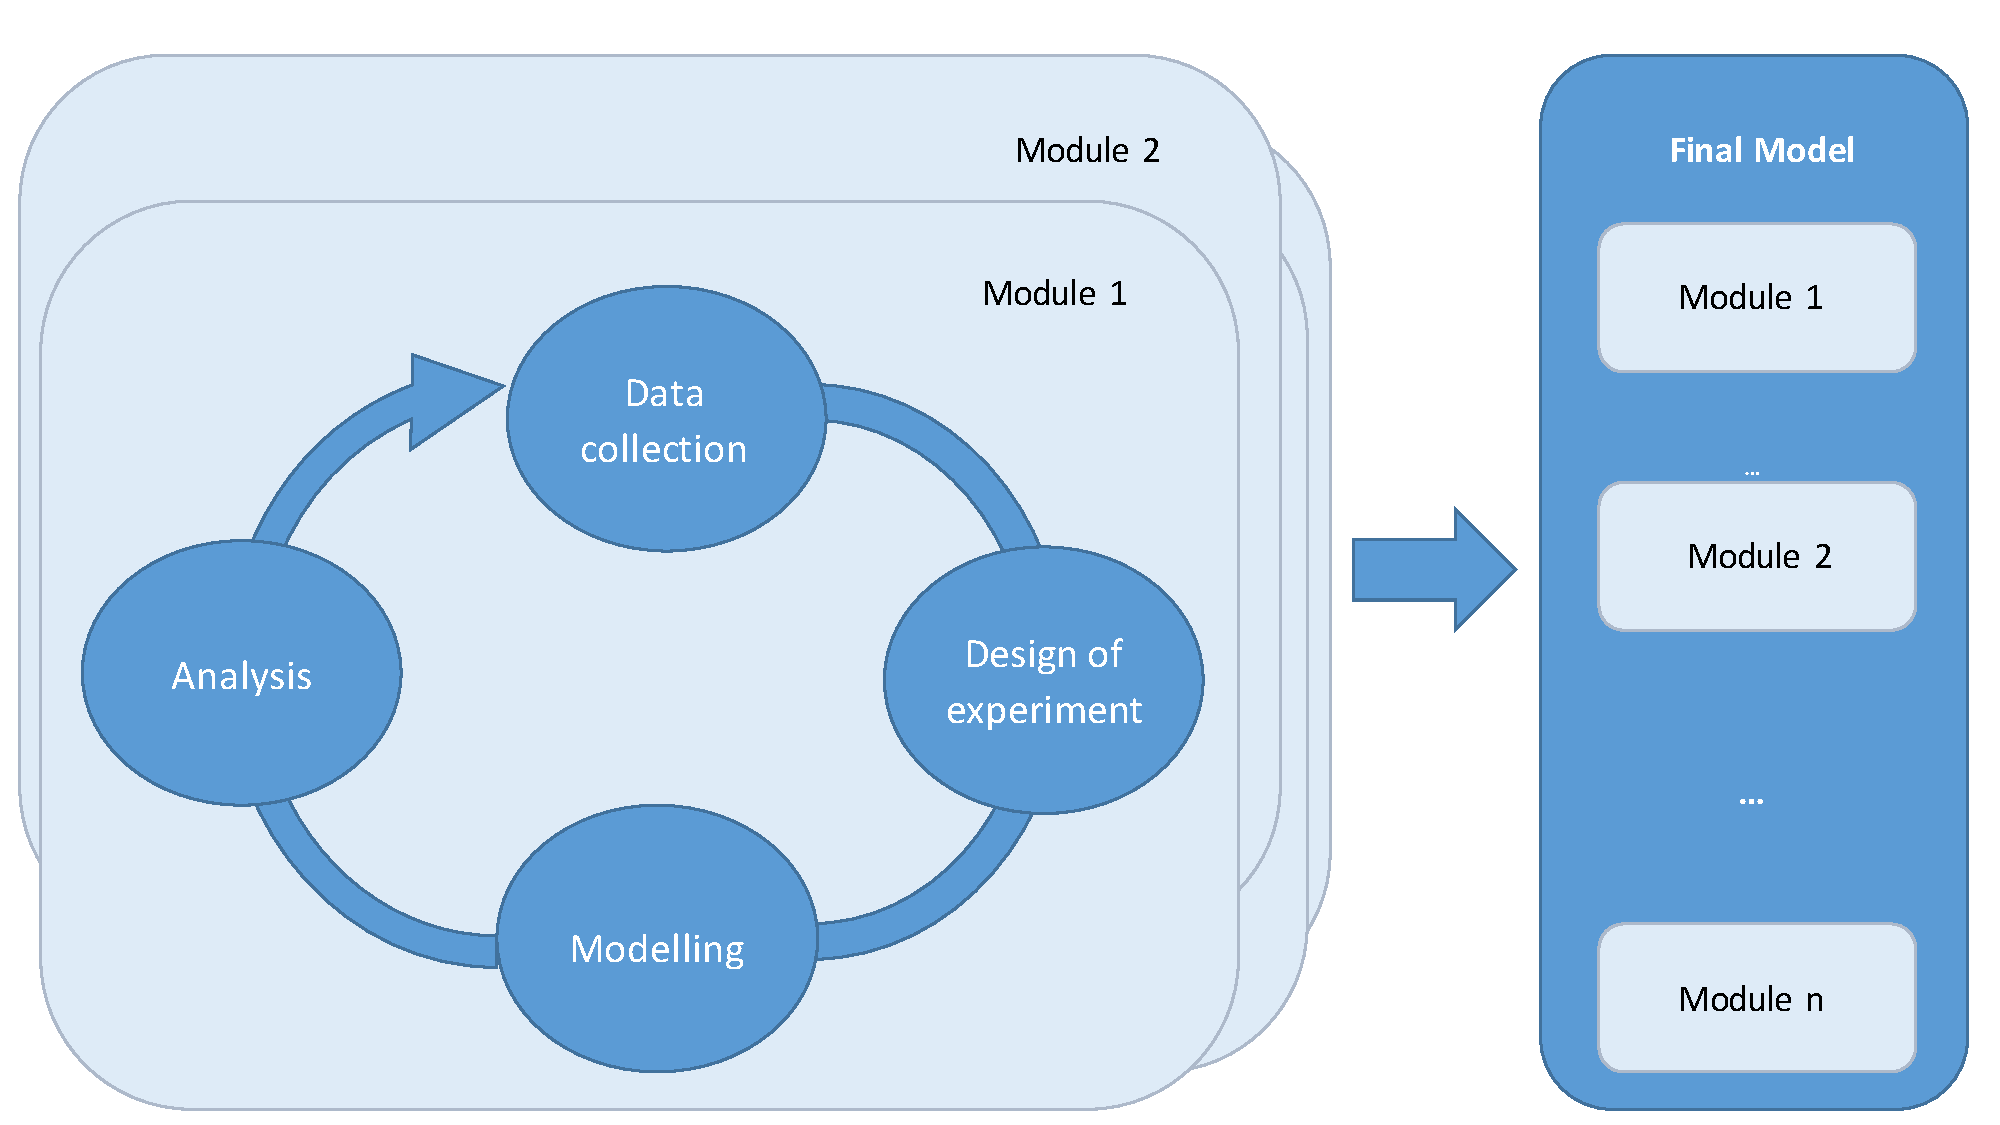
\includegraphics[width=\textwidth]{process}
\caption{Choosing the choice: An outline of the approach \label{fig:approach}}
\end{figure}

As argued throughout this Special Issue, all these features, and more, make agent-based modelling a very attractive analytical proposition for demographers. The potential gains in understanding of the underlying population processes cannot be overstated, and further links connecting agent-based and statistical demography are yet to be explored (see for example \citet{Bijak2016}). That at present there is no methodological consensus on modelling agency and human decisions is not an obstacle, but rather a challenge to guide the further work in this area. Given that over the last 15 years agent-based models have slowly begun to enter the demographic mainstream \citep{Billari2003,VanBavel2016}, the gaps in knowledge in the existing approaches have become clearly visible. In our view one of the important gaps is related to the agency and decision making processes of the simulated agents, and the related aspects, some of which – context, time, and a variety of forms of decision making – are discussed above. Now is the time to initiate the discussion about choosing the choice. 

\bibliography{choice}
\bibliographystyle{apacite}
\end{document}